\chapter{Arrays}
\renewcommand{\chaptertitle}{Arrays}

\lehead[]{\normalfont\sffamily\hspace*{-2.00cm}\textcolor{white}{\colorbox{lightblue}{\makebox[1.60cm][r]{\thechapter}}}\hspace{0.17cm}\textcolor{lightblue}{\chaptertitle}}
\rohead[]{\textcolor{lightblue}{\chaptertitle}\normalfont\sffamily\hspace*{0.17cm}\textcolor{white}{\colorbox{lightblue}{\makebox[1.60cm][l]{\thechapter}}}\hspace{-2.00cm}}
%\chead[]{}
\rehead[]{\textcolor{lightblue}{AvHG, Inf, My}}
\lohead[]{\textcolor{lightblue}{AvHG, Inf, My}}

\lstset{style=myJava}

Zur Verwaltung großer Mengen von Daten gibt es sogenannte \emph{Arrays}
(Datenfelder). Mit einer einzigen Array-Variablen kann man ein ganzes Feld von
Daten eines Datentyps verwalten.


\section{Arrays von primitiven Datentypen(boolean, int, double, char)}

\subsection{Eindimensionale Arrays}

\subsubsection{Deklaration (Anlegen der Variablen)}

\begin{lstlisting}
int[] zahl;
boolean[] wahr;
\end{lstlisting}

\subsubsection{Erzeugung des Datenfeldes}

\begin{lstlisting}
zahl = new int[200];                æ// erzeugt ein Feld mit Index 0 bis 199
æwahr = new boolean[2];              æ// erzeugt ein Feld mit Index 0 bis 1
\end{lstlisting}

\subsubsection{Deklaration und Erzeugung gleichzeitig}

\begin{lstlisting}
int[] zahlen = new int[15];         æ// erzeugt 15 int-Zahlen
æint[] liste = {10,3,12,3,5};        æ// erzeugt ein Array mit 5 int-Zahlen
æboolean[] b = {true, true, false};  æ// erzeugt ein Array mit 3 boolean-Werten
\end{lstlisting}

\subsubsection{Verwendung des Datenfeldes (einfache Datentypen)}

Bei einfachen Datentypen wie \lstinline|int| oder \lstinline|boolean|,
kann man die erzeugten Feldelemente über den Index ansprechen und Werte
hinein schreiben:

\begin{lstlisting}
for (int i = 0; i < 200; i++) {
    zahl[i] = 10 + i;
}
wahr[0] = false;
wahr[1] = true;
\end{lstlisting}

\subsubsection{Übergabe eines Arrays an eine Methode}

Aufruf der Methode:

\begin{lstlisting}
int summe1 = addieren(zahlen);
int summe2 = addieren(liste);
\end{lstlisting}

Deklaration der Methode:

\begin{lstlisting}
public int addieren (int[] feld) {
// addiert alle Zahlen des Feldes und gibt die Summe zurück
    int summe = 0;
    for (int i = 0; i < feld.length; i++) {
        summe += feld[i];
    }
    return summe;
}
\end{lstlisting}

Der Parameter \lstinline|feld| ist ein Array vom Typ \lstinline|int| von
beliebiger Länge. Es wird die Speicheradresse des Arrays übergeben, so dass sich
Änderungen im Array durch die Methode auch auf die übergebene Array-Variable
auswirken!

Das im Schleifenkopf benutzte Attribut \lstinline|feld.length| gibt die Länge
des Arrays an.


\subsection{Mehrdimensionale Arrays}

Beispiele:

\begin{lstlisting}
boolean[][] zweidimensional = new boolean[4][3];
zweidimensional[0][0] = true; 
zweidimensional[1][0] = false;
... 
zweidimensional[3][2] = false;

int[][][] dreidimensional = new int[20][3][4]; 
dreidimensional[19][2][3] = -97;
...
\end{lstlisting}


\section{Arrays von Objekten}

\subsubsection{Deklaration}

\begin{lstlisting}
Auto[] a;               æ// Variable vom Typ einer Klasse "Auto"
\end{lstlisting}

Es wird ein Speicherplatz angelegt, der später die Speicheradresse des
Datenfeldes speichern soll:

\begin{minipage}{0.15\textwidth}
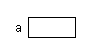
\includegraphics[width=1.0\textwidth]{./inf/SEKII/18_Java_Arrays/Deklaration.png}
\end{minipage}

\subsubsection{Erzeugung des Datenfeldes}

\begin{lstlisting}
a = new Auto[4];        æ// erzeugt Felder mit Index 0 bis 3
\end{lstlisting}

\begin{minipage}{0.45\textwidth}
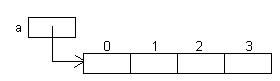
\includegraphics[width=1.0\textwidth]{./inf/SEKII/18_Java_Arrays/Erzeugung1.png}
\end{minipage}

\subsubsection{Erzeugung der Objekte}

Bei Feldern, die als Typ eine Klasse haben, muss man die einzelnen Objekte explizit erzeugen:

\begin{lstlisting}
a[0] = new Auto(10,20);
\end{lstlisting}

\begin{minipage}{0.45\textwidth}
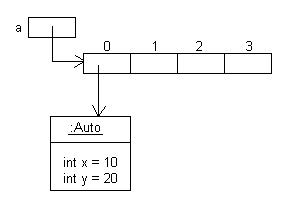
\includegraphics[width=1.0\textwidth]{./inf/SEKII/18_Java_Arrays/Erzeugung2.png}
\end{minipage}

Anschließend kann man Methoden und Variablen des Objektes aufrufen:

\begin{lstlisting}
a[0].x = 30;            æ// Verändert die Variable x des Objektes
æa[0].fahren(500);       æ// ruft die Methode "fahren" der Klasse Auto auf
\end{lstlisting}

\pagebreak

In einer Schleife kann man alle Objekte des Feldes auf einmal erzeugen:

\begin{lstlisting}
for (int x = 0; x < a.length; x++) {
    a[x] = new Auto(x*10, 20);
}
\end{lstlisting}

\begin{minipage}{0.6\textwidth}
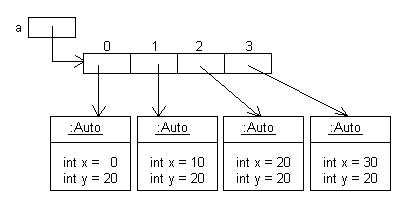
\includegraphics[width=1.0\textwidth]{./inf/SEKII/18_Java_Arrays/Erzeugung3.png}
\end{minipage}
